\documentclass[a4paper, notitlepage, 12pt]{scrartcl}
\author{Lukas Rost \\ \small{Teilnahme-ID: 48125}}
\title{Aufgabe 1 \\ \glqq Lisa rennt\grqq  - Dokumentation}
\subtitle{37. Bundeswettbewerb Informatik 2018/19 - 2. Runde \\~\\}
\date{29. April 2018}
\usepackage[ngerman]{babel}
\usepackage[utf8]{inputenc}
\usepackage{graphicx}
\usepackage{wrapfig}
\usepackage{color}
\usepackage[dvipsnames]{xcolor}
\usepackage{hyperref}
\usepackage[top=2.5cm, bottom=1.5cm, left=2.5cm, right=2.5cm]{geometry}
\usepackage{fancyvrb}
\usepackage{caption}
\usepackage{mathtools}
\usepackage{amssymb}
\usepackage{fancyhdr}
\usepackage{lastpage}

\usepackage{minted}
\fvset{breaklines=true}

\pagestyle{fancy}
\lhead{Lukas Rost, Teilnahme-ID: 48125}
\rhead{Aufgabe 1, Seite \thepage ~von \pageref{LastPage}}
\cfoot{ }

\newenvironment{longlisting}{\captionsetup{type=listing}}{}

\newmintedfile{kotlin}{frame=single,linenos,samepage=false,firstnumber=1,rulecolor=\color{Gray},autogobble,breakafter=.u,fontsize=\small}

\begin{document}
\renewcommand{\contentsname}{\centerline{Inhaltsverzeichnis}}
 \maketitle
 \tableofcontents
 \thispagestyle{empty}
 \newpage
 \setcounter{page}{1}
 
 \section{Lösungsidee}
 \subsection{Das Geometric-Shortest-Path-Problem}
 Das der Aufgabe zugrundeliegende Problem nennt sich \textit{Geometric Shortest Path} (GSP), auf Deutsch auch bekannt als Problem des geometrischen kürzesten Weges. Bei diesem Problem ist ein punktförmiger Roboter (oder auch eine Schülerin namens Lisa) gegeben, der/die sich an einer Startposition $p_{start}$ in einem kartesischen Koordinatensystem befindet. In diesem Koordinatensystem befinden sich mehrere als Polygone modellierte Hindernisse, wobei jedes einzelne Polygon durch seine Eckpunkte gegeben ist. Weiterhin ist eine Position $p_{ziel}$ gegeben. Nun soll ein möglichst kurzer Weg von $p_{start}$ zu $p_{ziel}$ gefunden werden, wobei dieser nicht durch Hindernisse führen soll.\footnote{Zumindest nicht, wenn Lisa als Zielposition nicht das Krankenhaus erreichen will.}\cite{Src:noem} \\ \\
 Das hier gegebene Problem unterscheidet sich von GSP dadurch, dass keine Position $p_{ziel}$, sondern eine Gerade $g_{ziel}$ (in Form eines beliebigen Punktes auf der Geraden) erreicht werden soll. Zusätzlich soll nicht unbedingt der Weg optimiert werden, sondern die Startzeit, die abhängig von der Länge des Weges und der für jeden Punkt der Geraden unterschiedlichen Zielzeit ist.
 [TODO labern bzgl. Problemstellung] \\ \\
 Das Geometric-Shortest-Path-Problem wird im Allgemeinen in zwei Schritten gelöst: Zunächst wird ein Sichtbarkeitsgraph erstellt, auf welchem dann Dijkstras Algorithmus ausgeführt wird. Zur Lösung des hier gegebenen Problems wird jedoch ein zusätzlicher Schritt benötigt, der auf der Lösung des Problems ohne Hindernisse basiert. Diese drei Algorithmen sollen in den folgenden Abschnitten vorgestellt und näher erläutert werden.
 \begin{figure}[H]
 	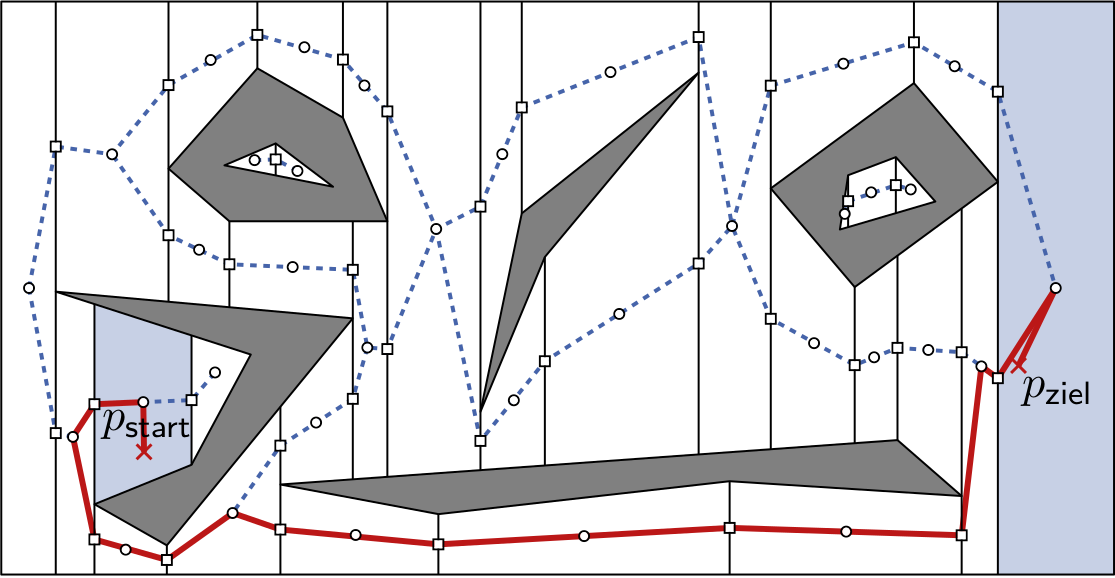
\includegraphics[scale=0.41]{pics/gsp}
 	\caption{Illustration des GSP-Problems (aus \cite{Src:noem})}
 \end{figure}
 \subsection{Erzeugung eines Sichtbarkeitsgraphen}
 \subsection{Der Dijkstra-Algorithmus}
 \subsection{Lösung des Problems ohne Hindernisse}
 \subsection{Kombination der Ansätze}
 \subsection{Laufzeitbetrachtung}
\begin{thebibliography}{xx}
\bibitem[1] {Src:bit} Bittel, O. (HTWG Konstanz): Autonome Roboter - Wegekartenverfahren, SS 2016 (Präsentation)
\bibitem[2] {Src:noem} Nöllenburg, Martin (KIT): Vorlesung Algorithmische Geometrie - Sichtbarkeitsgraphen, 2011 (Präsentation)
\bibitem[3]{Src:pyvis} Reksten-Monsen, Christian: Distance Tables Part 1 - Defining the Problem, \url{https://taipanrex.github.io/2016/09/17/Distance-Tables-Part-1-Defining-the-Problem.html}
\bibitem[4]{Src:pyvistwo} Reksten-Monsen, Christian: Distance Tables Part 2: Lee's Visibility Graph Algorithm, \url{https://taipanrex.github.io/2016/10/19/Distance-Tables-Part-2-Lees-Visibility-Graph-Algorithm.html}
\end{thebibliography}

\section{Umsetzung}
\subsection{Allgemeine Hinweise zur Benutzung}
\subsection{Struktur des Programms}
\subsection{Implementierung der wichtigsten Algorithmen}

\section{Beispiele}
\subsection{Beispiel 1}
\subsection{Beispiel 2}
\subsection{Beispiel 3}
\subsection{Beispiel 4}
\subsection{Beispiel 5}
\subsection{Eigene Beispiele}

 \section{Quellcode}
 \renewcommand{\listingscaption}{Quellcode}
 
 \end{document}